\documentclass{ercisbeamer}

\title{Effective Studying}
\subtitle{An Overview}
\author{Sven Ligensa}
\institute{European Research Center for Information Systems (ERCIS)}
\date{April 04, 2024}


\begin{document}

\setbgimage{00_resources/jungle_brain}
\begin{frame}
    \begin{tbox}
        \titlepage
        \begin{minipage}[c]{.32\textwidth}
            \centering
            \positive{\textbf{Link to LearnWeb course} \\ (HedgeDoc and slides) $\rightarrow$}
        \end{minipage}%
        \begin{minipage}[c]{.32\textwidth}
            
\includegraphics[height=.35\paperheight]{00_resources/qr_lw_course.png}
        \end{minipage}
    \end{tbox}
\end{frame}
\setbgimage{}

\section{Introduction}
\begin{frame}{Contents}
    \begin{itemize}
        \item \positive{\textbf{Introduction}}
        \item From \red{Science of Learning}…
        \begin{itemize}
            \item Illusions of Knowing
            \item Understanding the Brain
            \item Learning
            \item Desirable Difficulties
        \end{itemize}
        \item … to your \red{Learning Practice}
        \begin{itemize}
            \item Retrieval
            \item Spacing
            \item Variation \& Interleaving
            \item Mental Models
            \item Memory Cues
        \end{itemize}
        \item Recap
    \end{itemize}
\end{frame}

\begin{frame}{The Main Source}
    \begin{itemize}
        \item This material is based on the book \red{Make It Stick: The Science of Successful Learning}
        \begin{itemize}
            \item Available for free for students of the University of Münster \grey{(online in university network)} \\ \url{https://katalogplus.uni-muenster.de/permalink/49HBZ_ULM/1qrskqt/cdi_askewsholts_vlebooks_9780674419384}
            \item Contains lots of examples, based on numerous studies
        \end{itemize}
        \item Further sources are indicated when referenced
    \end{itemize}

    \begin{picture}(0,0)
        \put(300,-50){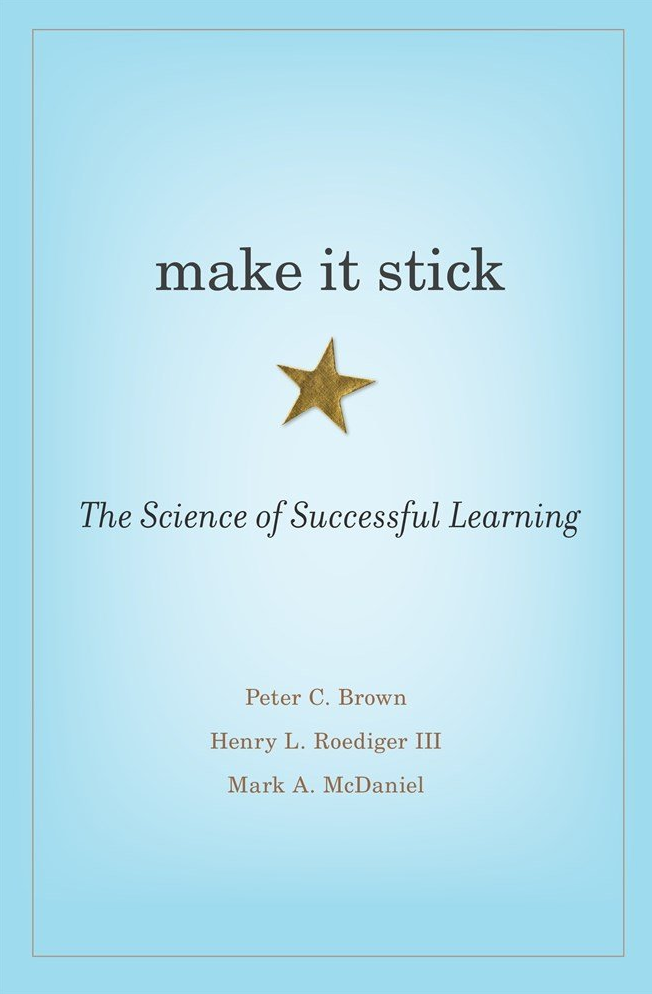
\includegraphics[width=0.15\paperwidth]{01_resources/makeitstick_frontpage.png}}
    \end{picture}
\end{frame}

\begin{frame}{Motivation: Why You Should Care}
    \begin{quote}
    If you're good at learning, you have an advantage in life. \grey{\textasciitilde{} Make It Stick, p. 2}
    \end{quote}
    \vspace{1em}
    \begin{itemize}
        \item Most of us don't really know how to learn effectively
        \begin{itemize}
            \item Striking quote: \emph{``Even in studies where the participants have \red{shown superior results from spaced learning}, they don't perceive the improvement; they \red{believe they learned better on the material where practice was massed.''} \grey{\textasciitilde{} Make It Stick, p. 47}}
            \item Same pattern for other effective study practices
        \end{itemize}
        \item But why is that so?
        \begin{itemize}
            \item Effective study strategies are often \red{not intuitive} at first glance
            \item It is \red{not} directly \red{taught} in school/university -- until now… ;)
        \end{itemize}
    \end{itemize}
\end{frame}

\begin{frame}{Objectives of Today's Session}
    \begin{itemize}
        \item Explain the underlying principles of how learning works
        \item Describe methods of effective studying; Apply selected ones during class
        \item Think about how to implement what you learned in your own study routines
    \end{itemize}
\end{frame}

\begin{frame}{Exam Hints}
    \begin{itemize}
        \item All information regarding exams can be found on the website of the \href{https://www.wiwi.uni-muenster.de/pam/en/examinations/schedule-examination-offer-examination-rooms}{examination office}
        \item Exams are (de-)registered and their results are published \href{https://pam-portal.uni-muenster.de/}{here}
        \item Exam phase \emph{directly} follows the lecture phase $\rightarrow$ Unavoidable to learn during lecture phase
        \item You have \emph{two attempts} to pass each examination in a module
        \begin{itemize}
            \item Additionally overall \emph{three third attempts}
        \end{itemize}
        \item Passed examinations cannot be repeated to improve grades
        \item Exams test \emph{transfer of knowledge}, not only reproduction
    \end{itemize}
\end{frame}

\begin{frame}{Trivial (?) Advice and Pointers}
    \begin{itemize}
        \item Go to the lectures, try to understand the topics while in class, ask questions
        \item Work on exercise sheets thoroughly; they usually foreshadow the types of tasks to be expected in the exam
        \item Keep track of your TODOs (e.g. via \href{https://todoist.com/}{Todoist}) and Deadlines (e.g. via \href{https://workspace.google.com/products/calendar/}{Google Calendar})
        \item Listening to music can make studying more enjoyable, but avoid music with lyrics: \\ E.g. \url{https://www.youtube.com/@AmbientWorlds}
        \item Past exams are available for most courses in the exam archive of the student council: \url{https://klausurarchiv.fachschaft-wiwi.ms/}
        \item This course \grey{(supervised by me)} provides more information on the topics: \url{https://sso.uni-muenster.de/LearnWeb/learnweb2/course/view.php?id=71370}
    \end{itemize}
\end{frame}

\begin{frame}{One Quick Question}
    \centering \emph{Which \red{learning strategies} do you know?}
\end{frame}

\section{Illusions of Knowing}
\begin{frame}{Contents}
    \begin{itemize}
        \item Introduction
        \item From \red{Science of Learning}…
        \begin{itemize}
            \item \positive{\textbf{Illusions of Knowing}}
            \item Understanding the Brain
            \item Learning
            \item Desirable Difficulties
        \end{itemize}
        \item … to your \red{Learning Practice}
        \begin{itemize}
            \item Retrieval
            \item Spacing
            \item Variation \& Interleaving
            \item Mental Models
            \item Memory Cues
        \end{itemize}
        \item Recap
    \end{itemize}
\end{frame}

\setbgimage{02_resources/feeling_ne_reality}
\begin{frame}{Illusions of Knowing | Overview}
    \begin{tbox}
        \begin{itemize}
            \item Fundamental difference: \red{Feeling $\ne$ Reality}
            \item Everyone is affected, often \negative{not} even \negative{aware}
            \item Fostered by \negative{ineffective learning strategies}
            \item Example of poor metacognition (judgement about what one knows)
            \item \red{Good metacognition}
            \begin{itemize}
                \item Critical for effective decision-making and learning
                \item Skill one must acquire
            \end{itemize}
        \end{itemize}
    \end{tbox}
\end{frame}

\begin{frame}{Illusions of Knowing | Familiarity Trap}
    \begin{tbox}
        \begin{itemize}
            \item Feeling that you know something
            \begin{itemize}
                \item[$\Rightarrow$] No longer need to practice it
                \item[$\Rightarrow$] Bad decisions on what to learn
            \end{itemize}
            
            \item \red{Fluency illusion}: Confuse: Fluency with text $\Leftrightarrow$ Mastery of its content
            \begin{itemize}
                \item \emph{Which learning strategy fosters this illusion? \pause $\rightarrow$ \negative{Rereading}}
            \end{itemize}
        \end{itemize}
    \end{tbox}
\end{frame}

\setbgimage{02_resources/mutable_memory}
\begin{frame}{Illusions of Knowing | Mutable Memory}
    \pause
    \begin{tbox}
        \begin{itemize}
            \item Memory = Reconstruction $\ne$ Reality
            \item Two-edged sword
            \begin{itemize}
                \item \negative{Skews our perceptions} \grey{$\Rightarrow$ Stay open to the fallibility of your certainties}
                \item \positive{Essential for learning}
            \end{itemize}
            \item \red{Hindsight Bias}: Tendency to overestimate how much one knew before an event happened $\Rightarrow$ Overconfidence
            \begin{itemize}
                \item \emph{How does it affect our studying? \pause $\rightarrow$ Coming into a tutorial session without working on the exercises beforehand $\Rightarrow$ Feeling that the exercises are easier than they actually are}
            \end{itemize}
            \item \red{Curse of Knowledge}: Tendency to underestimate how much time is needed for another person to learn something new or perform a task
            \begin{itemize}
                \item \emph{Where is this important in the university context? \pause $\rightarrow$ When teaching others, better schedule a bit more time (giving a presentation/tutorial)}
            \end{itemize}
        \end{itemize}     
    \end{tbox}
\end{frame}
\setbgimage{}

\begin{frame}{Illusions of Knowing | Remedies}
    \begin{itemize}
        \item \red{Effective learning strategies} like Retrieval
        \item \red{Objective ways} to track progress
        \item \red{``Practice like you play''}
        \item Practice with \red{others}
        \begin{itemize}
            \item Work alongside more skilled partner
            \item Seek corrective feedback
        \end{itemize}
        \item Be aware of what \red{criteria} you use to judge what you have learned
        \begin{itemize}
            \item \emph{What are good/bad criteria?} \pause
            \begin{itemize}
                \item \emph{\positive{Explaining} a text well using own words}
                \item \emph{\negative{Familiarity} with text}
            \end{itemize}
        \end{itemize}
    \end{itemize}
\end{frame}

\section{Understanding the Brain}
\begin{frame}{Contents}
    \begin{itemize}
        \item Introduction
        \item From \red{Science of Learning}…
        \begin{itemize}
            \item Illusions of Knowing
            \item \positive{\textbf{Understanding the Brain}}
            \item Learning
            \item Desirable Difficulties
        \end{itemize}
        \item … to your \red{Learning Practice}
        \begin{itemize}
            \item Retrieval
            \item Spacing
            \item Variation \& Interleaving
            \item Mental Models
            \item Memory Cues
        \end{itemize}
        \item Recap
    \end{itemize}
\end{frame}

\setbgimage{03_resources/neurons}
\begin{frame}{Understanding the Brain | Circuitry \& Neuroplasticity}
    \begin{tbox}
        \begin{itemize}
            \item \red{Neurons} communicating via \red{synapses} (connection between neurons)
            \begin{itemize}
                \item Enables: Senses, cognition, motor skills, learning, memory, …
                \item Forms possibilities and limits of person's intellectual capacity
            \end{itemize}
            \item \red{Neuroplasticity}: Brain is remarkably mutable (``plastic'')
            \begin{itemize}
                \item Learning $\Leftrightarrow$ Changing the brain
                \item Analogy: Backpropagation \grey{(used in Deep Learning)}
                \item Genes $\rightarrow$ Brain architecture (initialization point)
                \item Experience $\rightarrow$ Modification of fine structure
            \end{itemize}
        \end{itemize}
    \end{tbox}

    \begin{tbox}
        \begin{itemize}
            \item \citet{wieman12}: \red{Brain $\approx$ Muscle}
            \begin{itemize}
                \item ``The learning of \emph{complex expertise} is thus quite \emph{analogous to muscle development}. \\
                In response to the extended strenuous use of a muscle, it grows and strengthens. \\
                In a similar way, the brain changes and develops in response to its strenuous extended use.''
            \end{itemize}
        \end{itemize}
    \end{tbox}

    \begin{picture}(0,0)
        \put(359,104){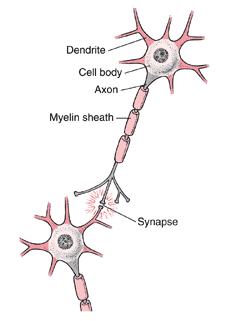
\includegraphics[width=0.179\paperwidth]{03_resources/neuron_schematic.png}}
    \end{picture}
    \begin{textblock*}{500pt}(0pt, -102pt)
        \tiny \url{https://www.researchgate.net/figure/Schematic-picture-of-two-neurons-Neurons-send-action-potentials-along-the-axon-which_fig1_41674066}
    \end{textblock*}
\end{frame}
\setbgimage{}

\begin{frame}{Understanding the Brain | Knowledge \& Memory}
    \begin{itemize}
        \item \red{Knowledge} and \red{memory} = Neural processes
        \begin{itemize}
            \item Maturation of connections = Gradual thickening of myelin coating of axons
            \item Practice $\Rightarrow$ Myelin$^\star$ $\uparrow$ $\Rightarrow$ Strength and speed of electrical signals $\uparrow$ \\ $\Rightarrow$ Performance $\uparrow$ ($\Rightarrow$ Motivation for further practice)
        \end{itemize}
        \item Actions taken by \red{habit} are directed from region located deeper in the brain
        \begin{itemize}
            \item Chunk sequence of steps to single unit $\Rightarrow$ Sequence becomes reflexive
            \item Examples: Finger movement of musicians, typing on a keyboard
            \item Analogy: Computer macro
        \end{itemize}
    \end{itemize}
    \begin{textblock*}{500pt}(145pt, 66pt)
        \tiny $^\star$\url{https://en.wikipedia.org/wiki/Myelin}
    \end{textblock*}
    
\end{frame}

\section{Learning}
\begin{frame}{Contents}
    \begin{itemize}
        \item Introduction
        \item From \red{Science of Learning}…
        \begin{itemize}
            \item Illusions of Knowing
            \item Understanding the Brain
            \item \positive{\textbf{Learning}}
            \item Desirable Difficulties
        \end{itemize}
        \item … to your \red{Learning Practice}
        \begin{itemize}
            \item Retrieval
            \item Spacing
            \item Variation \& Interleaving
            \item Mental Models
            \item Memory Cues
        \end{itemize}
        \item Recap
    \end{itemize}
\end{frame}

\setbgimage{04_resources/knowledge_spiral}
\begin{frame}{Learning | Overview}
    \begin{tbox}
        \begin{itemize}
            \item \red{Learning}: \emph{``\red{Acquiring knowledge} and skills and having them readily available from \red{memory} so you can make sense of \red{future} problems and opportunities.'' \grey{\textasciitilde{} Make It Stick, p. 2}}
            \item \emph{``If you're good at learning, you have an advantage in life.'' \grey{\textasciitilde{} Make It Stick, p. 2}}
            \begin{itemize}
                \item Need to keep learning and remembering \red{for life}
            \end{itemize}
            \item Getting information \red{out} of your brain, \negative{not in} \cite{agarwal19}
            \item \red{Iterative Process}: Revisiting knowledge like a spiral and understanding more every time
            \begin{itemize}
                \item \emph{Can you think of examples?} \pause
                \begin{itemize}
                    \item \emph{Reading a dense paper multiple times: \grey{Some aspects are immediately clear, others not. During the second reading, you build on top of the information have from the first reading.}}
                    \item \emph{Building up on knowledge about \emph{data} or \emph{processes} in subsequent modules: \grey{It would neither make sense to learn all the details in one module, nor to listen to subsequent modules first.}}
                    \item \emph{Refining your notes step-by-step to create a presentation}
                \end{itemize}
            \end{itemize}
            \item On neurological level: Strengthening neural pathways
            \item With right learning techniques: \red{No known limit to how much we can learn and remember if we relate it to what we already know}
        \end{itemize}
    \end{tbox}
\end{frame}

\setbgimage{04_resources/jungle_brain_50}
\begin{frame}{Learning | An Analogy}
    \begin{tbox}
        \begin{itemize}
            \item Knowledge $\widehat =$ \red{Tree} \grey{(hierarchical structure)} / \red{Network} \grey{(connections between nodes)}
            \begin{itemize}
                \item Connections: More = Better, Intense = Better
                \item \emph{Can you think of examples?} \pause \\ $\rightarrow$ \emph{Memory of your childhood neighborhood/accident}
            \end{itemize}
            \item New learning requires a foundation of \red{prior knowledge}
            \begin{itemize}
                \item Adding to tree of knowledge, requires existing knowledge to connect it to \\ $\rightarrow$ Make information digestible for you
            \end{itemize}
        \end{itemize}
    \end{tbox}
\end{frame}
\setbgimage{}

\begin{frame}{Learning | Forgetting}
    \begin{itemize}
        \item \red{Forgetting}: Inability to recall something (easily)
        \item Learning requires \red{memory}
        \item Central goal: Interrupt the \red{Forgetting Curve}
        \begin{itemize}
            \item We (exponentially) forget most information we consume after a short amount of time
        \end{itemize}
    \end{itemize}

    \begin{figure}
        \centering
        \includegraphics[width=0.35\paperwidth]{04_resources/forgetting_curve_remnote.png}
        \vspace{-0.5em}
        \caption{\tiny \url{https://www.remnote.com/assets/homepage/images/spaced_repetition_retention.webp}}
    \end{figure}
\end{frame}

\begin{frame}{Learning | The Role of Failure}
    \begin{itemize}
        \item Source of useful information
        \item Not desirable itself, but unavoidable $\rightarrow$ Effort despite risks
        \item Fear of failure $\Rightarrow$ Worse learning
        \item Important: \positive{Positive attitude} towards mistakes
        \item Few settings where failure not optimal learning strategy
        \begin{itemize}
            \item \emph{Can you think of an example?} \pause \emph{$\rightarrow$ Parachuting}
        \end{itemize}
    \end{itemize}
\end{frame}

\setbgimage{04_resources/own_your_learning}
\begin{frame}{Learning | Own Your Learning}
    \begin{tbox}
        \begin{itemize}
            \item \red{Elements shaping your intellectual abilities lie to a large extent within your own control}
            \item \red{Your learning = Your responsibility}
            \item Teachers are there to support you, but at the end, it is up to you how much you learn
        \end{itemize}
    \end{tbox}
\end{frame}
\setbgimage{}

\section{Desirable Difficulties}
\begin{frame}{Contents}
    \begin{itemize}
        \item Introduction
        \item From \red{Science of Learning}…
        \begin{itemize}
            \item Illusions of Knowing
            \item Understanding the Brain
            \item Learning
            \item \positive{\textbf{Desirable Difficulties}}
        \end{itemize}
        \item … to your \red{Learning Practice}
        \begin{itemize}
            \item Retrieval
            \item Spacing
            \item Variation \& Interleaving
            \item Mental Models
            \item Memory Cues
        \end{itemize}
        \item Recap
    \end{itemize}
\end{frame}

\setbgimage{05_resources/desirable_difficulties}
\begin{frame}{Desirable Difficulties | Overview}
    \begin{tbox}
        \begin{itemize}
            \item Desirable difficulties $\Rightarrow$ More effort during learning $\Rightarrow$ Deeper, more durable learning
            \item Can be overcome through \red{increased effort}
            \item Learning is \red{not} better when it's easier!
            \begin{itemize}
                \item \emph{``When learning is hard, you do important work.'' \grey{\textasciitilde{} Make It Stick, p. 7}}
                \item On the other hand: When it's easy, you could probably let it be
            \end{itemize}
            \item Feature of many \red{effective learning} strategies \grey{(Spacing, Interleaving, Variation, …)}
            \item \emph{Have you already experienced them in your own life?} \pause $\rightarrow$ \emph{In nearly every kind of sport training: Varying the kind of shot/throw/hit; Not practicing only few days before a match, but throughout the whole season}
        \end{itemize}
    \end{tbox}
\end{frame}
\setbgimage{}

\begin{frame}{Desirable Difficulties | Advantages and Disadvantages}
    \begin{itemize}
        \item \positive{Mimics challenges of practical experiences} \grey{($\rightarrow$ Practice like you play)}
        \item \positive{Help creating mental models} \grey{($\rightarrow$ Concepts, transfer)}
        \item \positive{Trigger encoding and retrieval processes}
        \item \negative{Feel less productive} \grey{($\rightarrow$ Illusions of Knowing)} \negative{$\Rightarrow$ Risk for motivation}
        \item \negative{Undesirable difficulties}: Cannot be overcome through increased effort
    \end{itemize}
\end{frame}

\section{Retrieval}
\begin{frame}{Contents}
    \begin{itemize}
        \item Introduction
        \item From \red{Science of Learning}…
        \begin{itemize}
            \item Illusions of Knowing
            \item Understanding the Brain
            \item Learning
            \item Desirable Difficulties
        \end{itemize}
        \item … to your \red{Learning Practice}
        \begin{itemize}
            \item \positive{\textbf{Retrieval}}
            \item Spacing
            \item Variation \& Interleaving
            \item Mental Models
            \item Memory Cues
        \end{itemize}
        \item Recap
    \end{itemize}
\end{frame}

\begin{frame}{Retrieval | Overview}
    \begin{itemize}
        \item \red{\textbf{Recalling already ``learned'' material from memory}}
        \begin{itemize}
            \item Works for facts, concepts, techniques, motor skills
        \end{itemize}
        \item Related terms: Active Recall, Practice Testing
        \item More than \red{100 years of research}
        \begin{itemize}
            \item \emph{``The active recall of a fact from within is, as a rule, better than its impression from without'' \grey{(Quote from the year 1906)}}
        \end{itemize}
        \item Does not need to be initiated by instructor $\rightarrow$ \red{Self-testing}
        \item Check answers $\rightarrow$ Combat Illusions of Knowing \grey{(Hindsight bias)}
        \begin{itemize}
            \item Important: Really \red{answer} the question before reviewing the solution
        \end{itemize}
        \item Restudying after failed retrieval $>$ Not attempting retrieval
        \item Knowledge harder to retrieve $\Rightarrow$ More benefit from retrieval
        \begin{itemize}
            \item Most effective in combination with \red{Spacing}
        \end{itemize}
    \end{itemize}
\end{frame}

\begin{frame}{Retrieval | Paradigm Shift}

    From: Tests are a necessary evil for \negative{measuring} learning
    
    \begin{picture}(0,120)
        \put(0, 0){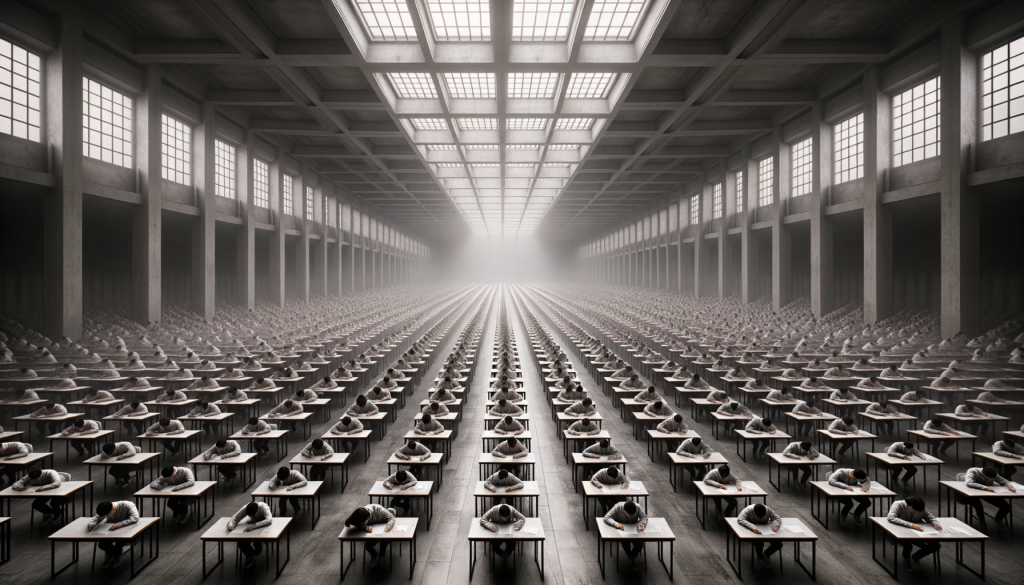
\includegraphics[width=0.45\paperwidth]{07_resources/exam}}
        \put(0.5\paperwidth, 0){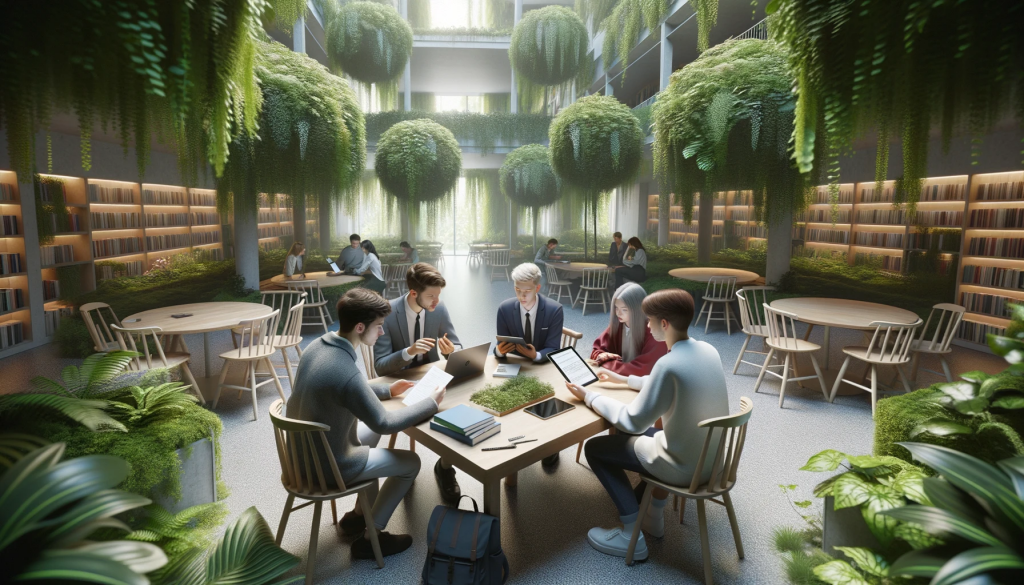
\includegraphics[width=0.45\paperwidth]{07_resources/study_group}}
    \end{picture}
    
    \hspace{17em} To: Tests can be a helpful tool for \positive{improving} learning
\end{frame}

\begin{frame}{Retrieval | Advantages}
    \begin{itemize}
        \item \positive{Strengthens memory}
        \item \positive{Shows gaps in knowledge} ($\rightarrow$ Combats Illusions of Knowing)
        \vspace{1em}
        \item Should be \red{primary study strategy}
        \begin{itemize}
            \item In combination with the other strategies we will cover on the following slides…
        \end{itemize}
    \end{itemize}
\end{frame}

\begin{frame}{Retrieval | Implementation}
    \begin{itemize}
        \item \red{Flashcards}
        \begin{itemize}
            \item Physical
            \item Digital
            \begin{itemize}
                \item Anki (\url{https://apps.ankiweb.net/})
                \item Phase 6 (\url{https://www.phase-6.de/})
                \item …
            \end{itemize}
        \end{itemize}
        \item \red{Questions + Answers}
        \begin{itemize}
            \item Physical
            \item Digital 
            \begin{itemize}
                \item Notion (\url{https://www.notion.so/product})
                \item Obsidian (\url{https://obsidian.md/})
                \item RemNote (\url{https://www.remnote.com/computer-science})
            \end{itemize}
        \end{itemize}
    \end{itemize}
\end{frame}

\begin{frame}{Retrieval | Now You!}
    \begin{itemize}
        \item \emph{What would you write on a simple flashcard to test yourself on the topic of Retrieval?} \pause
        \begin{itemize}
            \item \emph{Front: What is \red{Retrieval}?}
            \item \emph{Back: A very effective learning strategy where you answer a question instead of simply reading the solution}
        \end{itemize}
        \item \emph{Which of your courses benefit most from implementing Retrieval?}
        \item \emph{How exactly do you want to implement Retrieval into your study routine?}
    \end{itemize}
\end{frame}

\section{Spacing}
\begin{frame}{Contents}
    \begin{itemize}
        \item Introduction
        \item From \red{Science of Learning}…
        \begin{itemize}
            \item Illusions of Knowing
            \item Understanding the Brain
            \item Learning
            \item Desirable Difficulties
        \end{itemize}
        \item … to your \red{Learning Practice}
        \begin{itemize}
            \item Retrieval
            \item \positive{\textbf{Spacing}}
            \item Variation \& Interleaving
            \item Mental Models
            \item Memory Cues
        \end{itemize}
        \item Recap
    \end{itemize}
\end{frame}

\setbgimage{08_resources/spacing}
\begin{frame}{Spacing | Overview}
    \begin{tbox}
        \begin{itemize}
            \item \red{\textbf{Letting time pass between study sessions}}
            \item Leads to forgetting ($\rightarrow$ Forgetting Curve) = Desirable difficulty
            \item Anything you want to remember must be periodically recalled from memory
            \item Crucial aspect of everyday experiences
            \item Combine with Retrieval
            \item Reach back to retrieve prior material \\ $\rightarrow$ See how knowledge learned at different times \\ relate to each other
        \end{itemize}
        \vspace{3.5em} \hspace{0.1em}\\
    \end{tbox}
    \begin{picture}(0,0)
        \put(304,13.5){\includegraphics[width=0.3\paperwidth]{08_resources/forgetting_curve_remnote.png}}
    \end{picture}
    \begin{textblock*}{400pt}(185pt, -12pt)
        \tiny \url{https://www.remnote.com/assets/homepage/images/spaced_repetition_retention.webp}
    \end{textblock*}
\end{frame}

\begin{frame}{Spacing | Length of Interval}
    \begin{tbox}
        \begin{itemize}
            \item Enough that practice does not become mindless repetition
            \begin{itemize}
                \item Little forgetting should have set in
                \item Not so much that retrieval essentially involves relearning the material
            \end{itemize}
            \item Mastery of material $\uparrow$ $\Rightarrow$ Length of interval $\uparrow$
            \begin{itemize}
                \item Do not drop important information completely
            \end{itemize}
            \item Depends on study material
        \end{itemize}
    \end{tbox}
    
    \hspace{2em}
    
    \begin{tbox}
        \begin{itemize}
            \item \citet{karpicke11}
            \begin{itemize}
                \item \emph{``Repeated \red{spaced retrieval} had \red{powerful effects} on retention, but the \red{relative schedule} of repeated tests had \red{no discernible impact}.''}
                \item \emph{``It is well known that \red{increasing} the \red{absolute spacing} between repetitions \red{improves retention}, especially in the long term.''}
            \end{itemize}
        \end{itemize}
    \end{tbox}
\end{frame}
\setbgimage{}

\begin{frame}{Spacing | Advantages}
    \begin{itemize}
        \item Learning has time to \positive{consolidate} into cohesive representation in the brain for long-term memory
        \item \positive{Interrupts forgetting}
    \end{itemize}
\end{frame}

\begin{frame}{Spacing | Implementation}
    \begin{itemize}
        \item Set aside some time every week \red{throughout the semester} to study and \red{start early}
        \item Physical Flashcards: Manually (e.g. via Leitner system)
        \item Digital Flashcards: Implemented \red{algorithm} (can often be tuned for personal preference)
        \item Questions + Answers: \red{Revision calendar}
    \end{itemize}
\end{frame}

\begin{frame}{Spacing | Now You!}
    \begin{itemize}
        \item \emph{How exactly do you want to implement Spacing into your study routine? \\ Consider what works best with your Retrieval strategy.}
        \item \emph{When do you want to start studying for the next examination phase?}
        \item \emph{Apply spacing by reviewing this material in the next days.}
    \end{itemize}
\end{frame}

\section{Variation and Interleaving}
\begin{frame}{Contents}
    \begin{itemize}
        \item Introduction
        \item From \red{Science of Learning}…
        \begin{itemize}
            \item Illusions of Knowing
            \item Understanding the Brain
            \item Learning
            \item Desirable Difficulties
        \end{itemize}
        \item … to your \red{Learning Practice}
        \begin{itemize}
            \item Retrieval
            \item Spacing
            \item \positive{\textbf{Variation \& Interleaving}}
            \item Mental Models
            \item Memory Cues
        \end{itemize}
        \item Recap
    \end{itemize}
\end{frame}

\setbgimage{09_resources/variation}
\begin{frame}{Variation \& Interleaving | Overview}
    \begin{tbox}
        \begin{itemize}
            \item \red{\textbf{Variation}}: \red{Vary the exercises you engage in}
            \begin{itemize}
                \item On level of individual topic
            \end{itemize}
            \item \red{\textbf{Interleaving}}: \red{Interleave practice of multiple topics/subjects/skills}
            \begin{itemize}
                \item On level of multiple topics
                \item Switch \red{before} each practice is complete
                \item Alternate between different problems that need different solutions $\Rightarrow$ Need to recognize problem type first, then select right solution
            \end{itemize}
            \item Antipattern: \negative{Blocked} practice
            \begin{itemize}
                \item Still widespread in school and university
            \end{itemize}
        \end{itemize}
    \end{tbox}
\end{frame}
\setbgimage{}

\begin{frame}{Variation \& Interleaving | Advantages}
    \begin{itemize}
        \item \positive{Versatility} of learning
        \begin{itemize}
            \item Finding commonalities/differences between different problems
            \item \positive{Broader understanding}
            \item \positive{Better assessment of context} and \positive{selecting right solution}
            \item \positive{Transfer of learning} between situations
        \end{itemize}
        \item Interleaving further implements Spacing $\Rightarrow$ Retrieval is harder
    \end{itemize}
\end{frame}

\begin{frame}{Variation \& Interleaving | Implementation}
    \begin{itemize}
        \item Vary the exercises $\rightarrow$ E.g. \red{Mock exams}
        \item \red{Shuffle} your flashcards
        \item Create \red{study plan} for which topic to study when \grey{(needs a bit more foresight)}
    \end{itemize}
\end{frame}

\begin{frame}{Variation \& Interleaving | Now You!}
    \begin{itemize}
        \item \emph{How exactly do you want to implement Variation and Interleaving into your study routine?}
        \item \emph{Do you want to create a study plan for the next examination phase?}
    \end{itemize}
\end{frame}

\section{Mental Models}
\begin{frame}{Contents}
    \begin{itemize}
        \item Introduction
        \item From \red{Science of Learning}…
        \begin{itemize}
            \item Illusions of Knowing
            \item Understanding the Brain
            \item Learning
            \item Desirable Difficulties
        \end{itemize}
        \item … to your \red{Learning Practice}
        \begin{itemize}
            \item Retrieval
            \item Spacing
            \item Variation \& Interleaving
            \item \positive{\textbf{Mental Models}}
            \item Memory Cues
        \end{itemize}
        \item Recap
    \end{itemize}
\end{frame}

\begin{frame}{Mental Models | Overview}
    \begin{tbox}
        \begin{itemize}
            \item \red{\textbf{Deeply entrenched and highly efficient skills or knowledge structures}}
            \begin{itemize}
                \item Interrelated concepts \grey{(or sequence of motor skills)}
                \item \red{Connected}: Fused into \red{meaningful whole}
            \end{itemize}
            \item Mental representation of (key ideas/underlying principles/rules from) external reality (learning material)
            \begin{itemize}
                \item Differentiate: Salient concepts vs. Unimportant details
            \end{itemize}
            \item Arise and improve through \red{effortful practice}
            \item Important: Ability to discern when our mental models are \negative{not} working
            \item Conscious or subconscious
            \item Connected with other mental models (prior knowledge)
            \item Adaptability and applicability in various circumstances
            \item Metaphors can deliver structure to build mental model
        \end{itemize}
    \end{tbox}
\end{frame}

\setbgimage{10_resources/mental_model}
\begin{frame}{Mental Models | Analogies \& Examples}
    \begin{tbox}
        \begin{itemize}
            \item Map, framework
            \item \red{Code library}: Library of myriad useful solutions that we can call on at will
        \end{itemize}
    \end{tbox}

    \vspace{.5em}

    \begin{tbox}
        \begin{itemize}
            \item \emph{Can you think of examples?} \pause
            \begin{itemize}
                \item Motor skills
                \begin{itemize}
                    \item Driving a car
                    \item Typing on a keyboard
                    \item Hitting a ball with a racket
                    \item Performing a muscle up
                \end{itemize}
                \item Cognitive skills
                \begin{itemize}
                    \item Knowing a topic inside out and being able to reference it a will (e.g. knowing characteristics of a process or how parts of a complex system interact with each other)
                \end{itemize}
            \end{itemize}
        \end{itemize}    
    \end{tbox}
\end{frame}

\setbgimage{10_resources/outline}
\begin{frame}{Mental Models | Make the Material Your Own}
    \begin{tbox}
        \begin{itemize}
            \item Actively \red{question} the \red{structure} of the presented material and \red{restructure} it as needed (also overarching multiple lecture sessions or even modules)
            \begin{itemize}
                \item It may be the most logical for the lecturer, but not for you
                \item Everybody thinks a bit differently
                \item They may be impacted by the \emph{Curse of Knowledge}
                \item After all, it has to make sense for \emph{you}
            \end{itemize}
        \end{itemize}
    \end{tbox}
\end{frame}
\setbgimage{}

\begin{frame}{Mental Models | Advantages}
    \begin{itemize}
        \item More successful at \positive{selecting right solution} for unfamiliar problems
        \begin{itemize}
            \item Extremely important for knowledge workers
            \item In current times: While AI tools \grey{(like ChatGPT)} can aid with many retrieval tasks, they will not be able to replace your mental models \grey{(in the foreseeable future)}
        \end{itemize}
        \item Results in \positive{conceptual knowledge} ($=$ understanding relationships of of basic elements within larger structure) instead of factual knowledge
    \end{itemize}
\end{frame}

\setbgimage{10_resources/big_picture}
\begin{frame}{Mental Models | Implementation}
    \begin{tbox}
        \begin{itemize}
            \item Distil information into ``\red{Big Picture}''
            \begin{itemize}
                \item Contains overview, interrelation of topics, general insights
            \end{itemize}
            \item Test yourself on key concept
            \begin{itemize}
                \item Be able to \red{define} it (in own words) and \red{use} it
                \item Also for \red{mathematical formulas}
            \end{itemize}
        \end{itemize}
    \end{tbox}
\end{frame}
\setbgimage{}

\begin{frame}{Mental Models | Now You!}
    \begin{itemize}
        \item \emph{Which of your courses benefit most from creating Mental Models?}
        \item \emph{Do you want to create Big Pictures? Or do you think other methods can be more efficient?}
        \item \emph{How---if at all---can you effectively combine the Big Picture and Retrieval?}
    \end{itemize}
\end{frame}

\section{Memory Cues}
\begin{frame}{Contents}
    \begin{itemize}
        \item Introduction
        \item From \red{Science of Learning}…
        \begin{itemize}
            \item Illusions of Knowing
            \item Understanding the Brain
            \item Learning
            \item Desirable Difficulties
        \end{itemize}
        \item … to your \red{Learning Practice}
        \begin{itemize}
            \item Retrieval
            \item Spacing
            \item Variation \& Interleaving
            \item Mental Models
            \item \positive{\textbf{Memory Cues}}
        \end{itemize}
        \item Recap
    \end{itemize}
\end{frame}

\setbgimage{11_resources/massive_information}
\begin{frame}{Memory Cues | Overview}
    \begin{tbox}
        \begin{itemize}
            \item Something with \red{\textbf{familiar structure to link information to}}
            \item Mental framework to store and later recall (large amounts of) information
            \item Organize what is already learned: \red{Understanding} first, \red{remembering} second!
            \begin{itemize}
                \item Should \red{\textbf{not}} be used to skip the understanding phase
            \end{itemize} 
            \item After repeated usage, not needed anymore
            \item \emph{Can you think of an example?} \pause
            $\rightarrow$ \red{P}lease \red{D}o \red{N}ot \red{T}hrow \red{S}ausage \red{P}izza \red{A}way \grey{(Seven layers of ISO OSI model)}
        \end{itemize}
    \end{tbox}
\end{frame}
\setbgimage{}

\begin{frame}{Memory Cues | Advantages}
    \begin{itemize}
        \item Commit \positive{huge} amounts of information to memory that have \positive{little to no connection}
    \end{itemize}
\end{frame}

\section{Recap}
\begin{frame}{Contents}
    \begin{itemize}
        \item Introduction
        \item From \red{Science of Learning}…
        \begin{itemize}
            \item Illusions of Knowing
            \item Understanding the Brain
            \item Learning
            \item Desirable Difficulties
        \end{itemize}
        \item … to your \red{Learning Practice}
        \begin{itemize}
            \item Retrieval
            \item Spacing
            \item Variation \& Interleaving
            \item Mental Models
            \item Memory Cues
        \end{itemize}
        \item \positive{\textbf{Recap}}
    \end{itemize}
\end{frame}

\begin{frame}{Recap | Effective vs. Ineffective Learning Strategies}
    \renewcommand{\arraystretch}{1.3}
    \begin{table}[h]
        \begin{tabularx}{\textwidth}{|>{\centering\arraybackslash}X|>{\centering\arraybackslash}X|>{\centering\arraybackslash}X|}
        \hline
        \Large\textbf{\red{Aspect}} & \Large\textbf{\red{Ineffective}} & \Large\textbf{\red{Effective}} \\
        \hline
        \red{Popular? Intuitive?} & \multirow{2}{*}{\centering Yes$^\star$} & \multirow{2}{*}{\centering No} \\
        \red{Feel productive?} & & \\
        \hline
        \red{Developed} & \negative{Momentary} & Underlying \positive{habit} strength \\
        \red{strength} & strength & \grey{$\rightarrow$ ``Mastery''} \\
        \hline
        \red{Desirable Difficulties} & \negative{Not implemented} & \positive{Implemented} \\
        \hline
        \red{Illusions of Knowing} & \negative{Promoted} & \positive{Counterbalanced} \\
        \hline
        \red{Primary mode} & \negative{Passive} & \positive{Active} \\
        \hline
        \multicolumn{3}{|c|}{\footnotesize $^\star$Even when people know about effective learning strategies, some still prefer ineffective ones!} \\
        \hline
        \end{tabularx}
    \end{table}
\end{frame}

\thankyou{Happy Learning!}{sven.ligensa@uni-muenster.de}

\sources

\begin{frame}{Link to LearnWeb Course and Slides}
    \centering 
\includegraphics[height=.85\paperheight]{00_resources/qr_lw_course.png}
\end{frame}

\end{document}
